\documentclass[fleqn]{article}

\usepackage[nodisplayskipstretch]{setspace}
\usepackage{amsmath, nccmath}
\usepackage{amssymb}
\usepackage{enumitem}
\usepackage{float}
\usepackage{graphicx}

\title{Homework 1}
\author{Owen Sowatzke}
\date{September 19, 2023}

\begin{document}
	\setlength{\abovedisplayskip}{0pt}
	\setlength{\belowdisplayskip}{0pt}
	\setlength{\abovedisplayshortskip}{0pt}
	\setlength{\belowdisplayshortskip}{0pt}
	\setlength{\mathindent}{0pt}
	\doublespacing
	\maketitle
	
	\begin{enumerate}[nolistsep]
		\item[1.] Use the graphical method to convolve the following signals. I.e., flip one signal and slide it across the other signal. Show graphs to illustrate your steps.
		
		$h[n] = 0.5\delta[n] - 0.25\delta[n-1]$
		
		$x[n] = (n+1)u[n]u[2-n]$
		
		The convolution output $y[n]$ is given by the following formula:
		
		\begin{align*}
			y[n] = \sum_{k=-\infty}^{\infty}{x[k]h[n-k]}
		\end{align*}
		
		To graphically convolve the signals, we need to form plots of $x[k]$ and \newline $h[n-k]$. The output $y[n]$ can be generated for each value of $n$ by multiplying $x[k]$ with $h[n-k]$ and summing the result.
		
		Start by plotting $x[n]$ and $h[n]$ as illustrated in Figure \ref{prob1_xn_plot} and in Figure \ref{prob1_hn_plot} respectively.
		
		\begin{figure}[H]				
			\centerline{\fbox{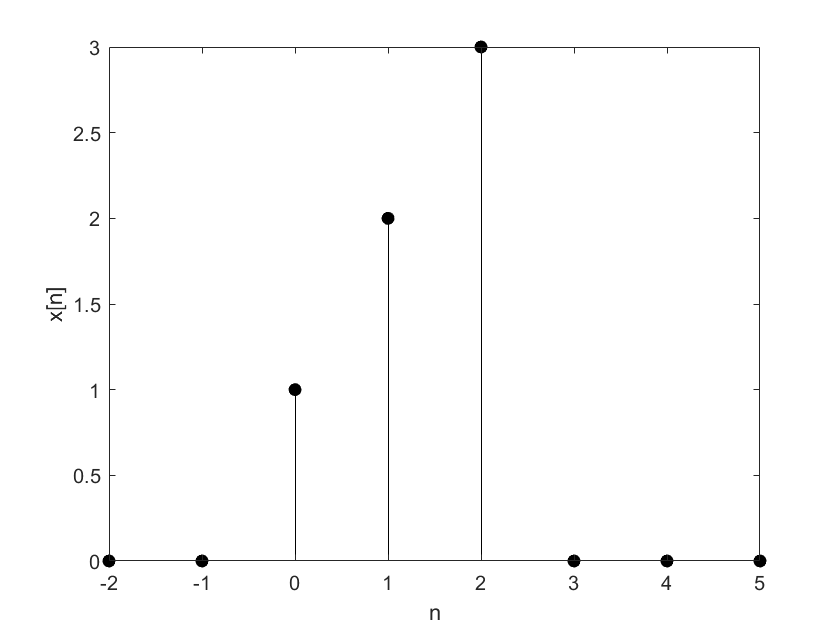
\includegraphics[width=0.5\textwidth]{prob1_xn_plot.png}}}
			\caption{Plot of $x[n]$}
			\label{prob1_xn_plot}
		\end{figure}
		
		\begin{figure}[H]				
			\centerline{\fbox{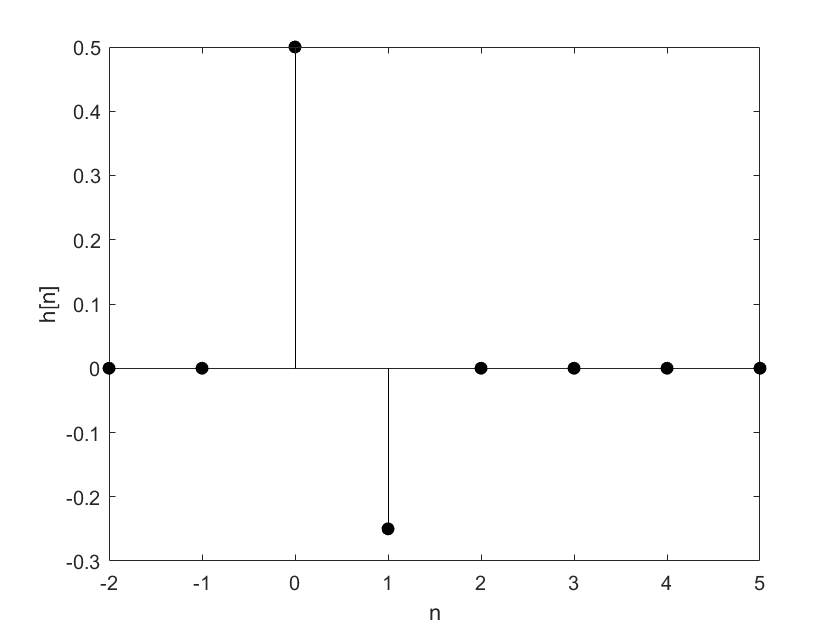
\includegraphics[width=0.5\textwidth]{prob1_hn_plot.png}}}
			\caption{Plot of $h[n]$}
			\label{prob1_hn_plot}
		\end{figure}
		
		Next, plot $x[k]$ and $h[k]$ as illustrated in Figure \ref{prob1_xk_plot} and Figure \ref{prob1_hk_plot} respectively. 
		
		\begin{figure}[H]				
			\centerline{\fbox{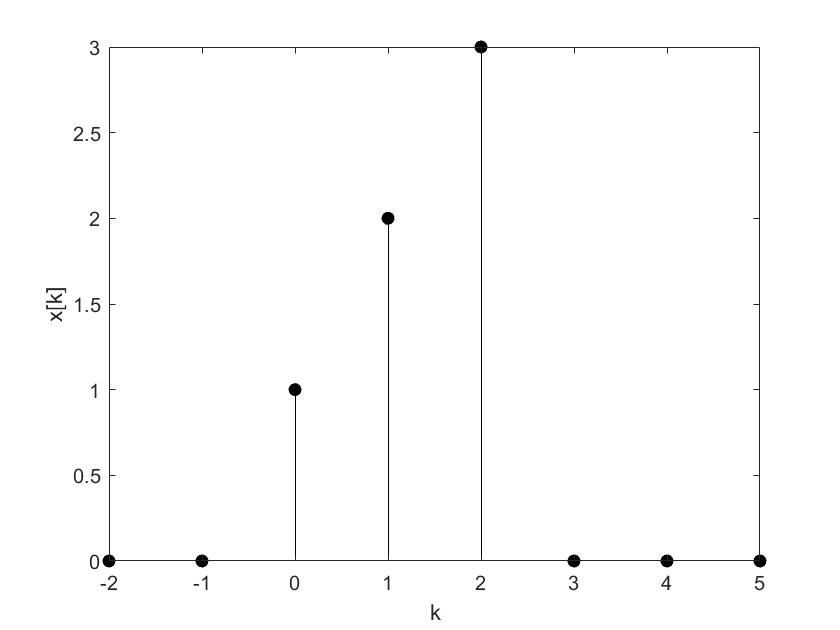
\includegraphics[width=0.5\textwidth]{prob1_xk_plot.png}}}
			\caption{Plot of $x[k]$}
			\label{prob1_xk_plot}
		\end{figure}
		
		\begin{figure}[H]				
			\centerline{\fbox{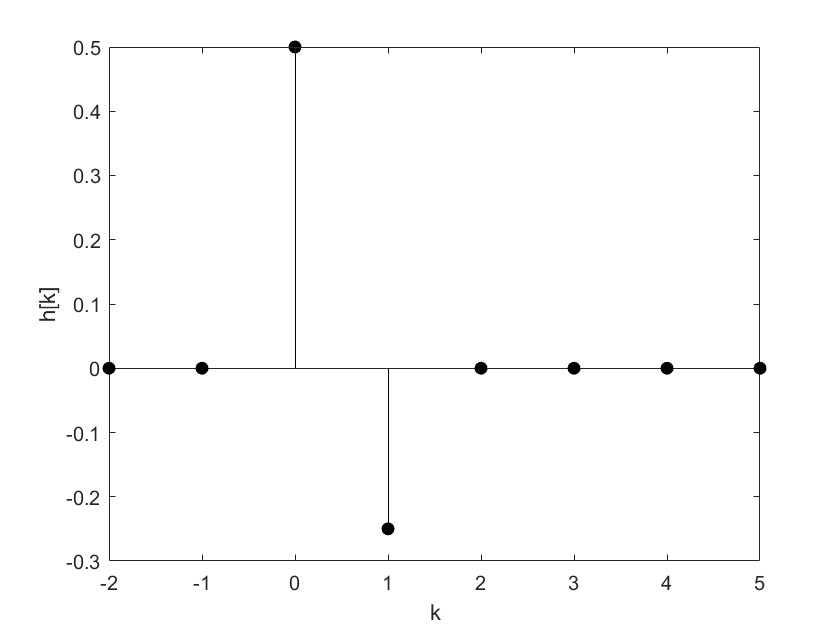
\includegraphics[width=0.5\textwidth]{prob1_hk_plot.png}}}
			\caption{Plot of $h[k]$}
			\label{prob1_hk_plot}
		\end{figure}
		
		Then, flip $h[k]$ to obtain $h[-k]$ and plot the result as shown in Figure \ref{prob1_h-k_plot}.
		
		\begin{figure}[H]				
			\centerline{\fbox{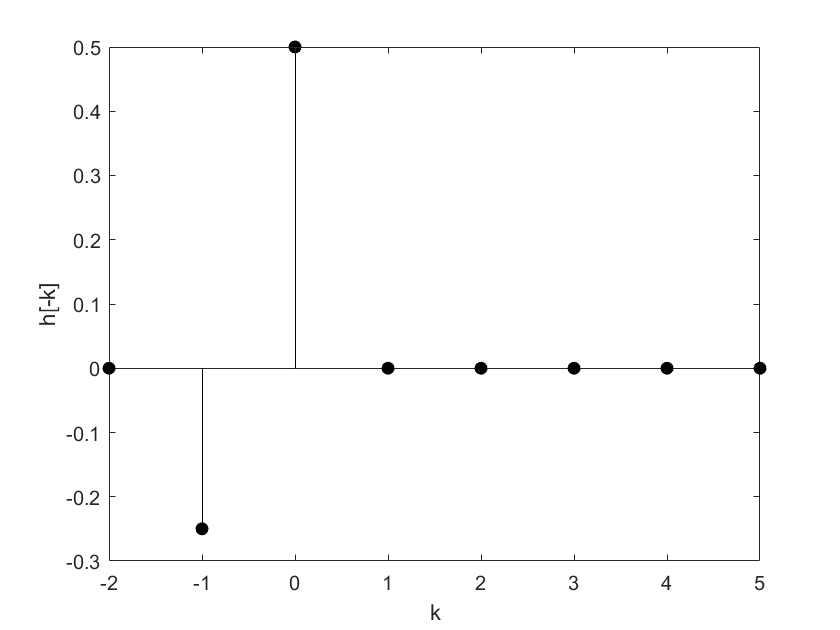
\includegraphics[width=0.5\textwidth]{prob1_h-k_plot.png}}}
			\caption{Plot of $h[-k]$}
			\label{prob1_h-k_plot}
		\end{figure}
		
		Now, shift $h[-k]$ by $n$ to obtain $h[n-k]$ and plot the result as shown in Figure \ref{prob1_hn-k_plot}.
		
		\begin{figure}[H]				
			\centerline{\fbox{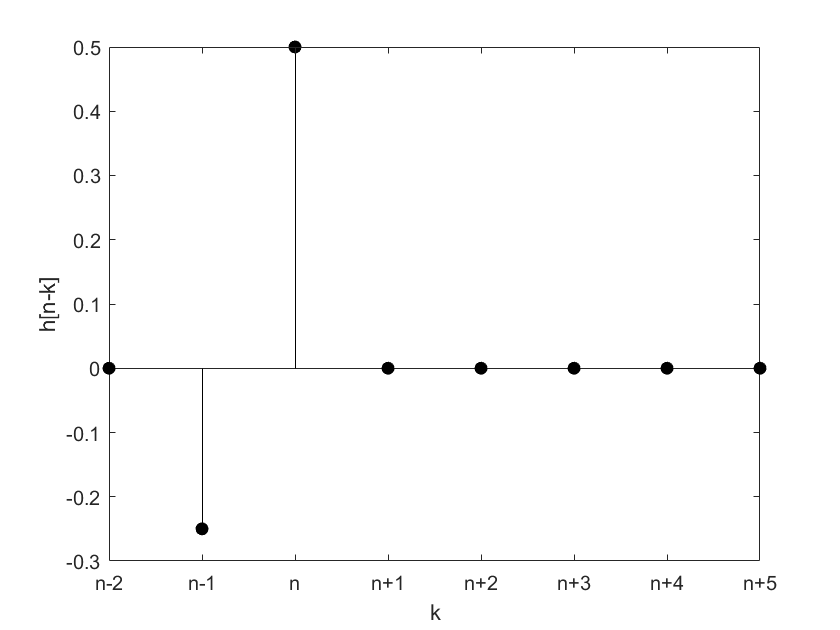
\includegraphics[width=0.5\textwidth]{prob1_hn-k_plot.png}}}
			\caption{Plot of $h[n-k]$}
			\label{prob1_hn-k_plot}
		\end{figure}
		
		For each value of $n$, multiply $x[k]$ by $h[n-k]$ and sum the result.
		
		For $n < 0$:
		
		$y[n] = 0$
		
		$y[0] = 0.5(1) = 0.5$
		
		$y[1] = 0.5(2) - 0.25(1) = 1 - 0.25 = 0.75$
		
		$y[2] = 0.5(3) - 0.25(2) = 1.5 - 0.5 = 1$
		
		$y[3] = -0.25(3) = -0.75$
		
		For $n > 3$:
		
		$y[n] = 0$:
		
		$\mathbf{\therefore y[n] = 0.5\delta[n] + 0.75\delta[n-1] + \delta[n-2] - 0.75\delta[n-3]}$
		
		The result $y[n]$ is plotted in Figure \ref{prob1_yn_plot}.
		
		\begin{figure}[H]				
			\centerline{\fbox{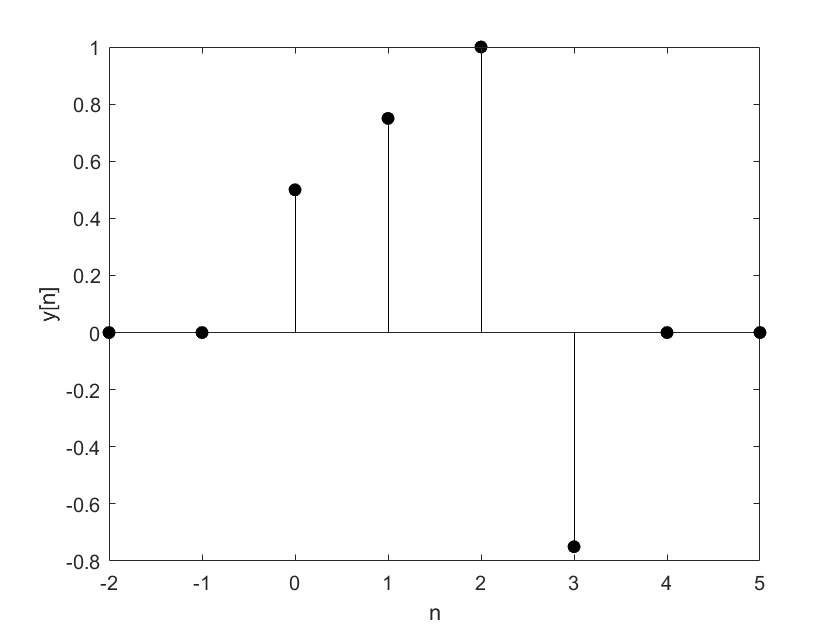
\includegraphics[width=0.5\textwidth]{prob1_yn_plot.png}}}
			\caption{Plot of $y[n]$}
			\label{prob1_yn_plot}
		\end{figure}
		
		\item[2.] Evaluate the convolution sum mathematically (i.e., do not use the graphical method) to obtain the unit step response of an LTI system whose impulse response is
		
		$h[n] = 3^{-n}u[n]$
		
		\begin{align*}
			y[n] = \sum_{k = -\infty}^{\infty}{x[k]h[n-k]} = \sum_{k = -\infty}^{\infty}{h[k]x[n-k]} = \sum_{k = -\infty}^{\infty}{3^{-k}u[k]u[n-k]}
		\end{align*}
		
		\begin{align*}
			= \sum_{k = 0}^{\infty}{3^{-k}u[n-k]}
		\end{align*}
		
		For $n < 0$:
		
		$y[n] = 0$
		
		\break
		
		For $n \geq 0$:
		
		\begin{align*}
			y[n] = \sum_{k = 0}^{n}{3^{-k}} = \sum_{k = 0}^{n}{(3^{-1})^k} = \sum_{k = 0}^{n}{\left(\frac{1}{3}\right)^k} = \frac{1-\left(\frac{1}{3}\right)^{n+1}}{1-\frac{1}{3}}
		\end{align*}
		
		\begin{align*}
			 = \frac{3\left(1-\left(\frac{1}{3}\right)^{n+1}\right)}{3\left(1-\frac{1}{3}\right)} = \frac{3-3\left(\frac{1}{3}\right)^{n+1}}{3-1} = \frac{3-\left(\frac{1}{3}\right)^{n}}{2} = \frac{1}{2}\left(3-\left(\frac{1}{3}\right)^{n}\right)
		\end{align*}
		
		\begin{align*}
			\mathbf{\therefore y[n] = \frac{1}{2}\left(3-\left(\frac{1}{3}\right)^{n}\right)u[n]}
		\end{align*}
		
		\item[3.] Consider three LTI systems having the following respective impulse responses:
		
			\begin{enumerate}[nolistsep]
				\item[(a)] $h[n] = 0.5\delta[n] + 0.2u[n-1]$
				
				\item[(b)] $h[n] = 3^{-n}u[n+1]$
				
				\item[(c)] $h[n] = 0.2u[n+2]u[2-n]$
				
			\end{enumerate}
			
			For each system, determine whether the system is (1) causal and (2) stable, and complete the following table:
			
			\begin{center}
				\begin{tabular}{|c|c|c|}
					\hline
					& Causal? (Yes/No) & Stable? (Yes/No) \\
					\hline
					(a) & & \\
					\hline
					(b) & & \\
					\hline
					(c) & & \\
					\hline
				\end{tabular}
			\end{center}
			
			\begin{enumerate}[nolistsep]
				\item[(a)] $h[n] = 0.5\delta[n] + 0.2u[n-1]$
				
					$h[n]$ is causal iff $h[n] = 0\ \forall\ n < 0$.
					
					$h[n] = 0\ \forall\ n < 0$.
					
					$\therefore h[n]$ is causal.
					
					$h[n]$ is stable iff $h[n]$ is absolutely summable.
					
					\begin{align*}
						\sum_{n=-\infty}^{\infty}{|h[n]|} = \sum_{n=-\infty}^{\infty}{|0.5\delta[n] + 0.2u[n-1]|}
					\end{align*}
					
					\begin{align*}
						= \sum_{n=-\infty}^{\infty}{0.5\delta[n] + 0.2u[n-1]} = \sum_{n=-\infty}^{\infty}{0.5\delta[n]} + \sum_{n=-\infty}^{\infty}{0.2u[n-1]}
					\end{align*}
				
					\begin{align*}
						= 0.5 + \sum_{n=1}^{\infty}{0.2} = \infty
					\end{align*}
				
					$h[n]$ is not absolutely summable.
				
					$\therefore h[n]$ is not stable.
				
				\item[(b)] $h[n] = 3^{-n}u[n+1]$
				
					$h[n]$ is causal iff $h[n] = 0\ \forall\ n < 0$.
					
					$h[-1] = 3^{-(-1)} = 3 \neq 0$.
					
					$\therefore h[n]$ is not causal.
					
					$h[n]$ is stable iff $h[n]$ is absolutely summable.
					
					\begin{align*}
						\sum_{n=-\infty}^{\infty}{|h[n]|} = \sum_{n=-\infty}^{\infty}{|3^{-n}u[n+1]|} = \sum_{n=-\infty}^{\infty}{3^{-n}u[n+1]} = \sum_{n=-1}^{\infty}{3^{-n}}
					\end{align*}
					
					Let $m = n - 1 \Rightarrow n = m + 1$
					
					\begin{align*}
						\sum_{n=-\infty}^{\infty}{|h[n]|} = \sum_{m=0}^{\infty}{3^{-(m+1)}} = 3^{-1}\sum_{m=0}^{\infty}{3^{-m}} = \frac{1}{3}\sum_{m=0}^{\infty}{(3^{-1})^{m}}
					\end{align*}
					
					\begin{align*}
						 = \frac{1}{3}\sum_{m=0}^{\infty}{\left(\frac{1}{3}\right)^{m}}
					\end{align*}
					
					Note this summation is of the form:
					
					\begin{align*}
						\sum_{n=0}^{\infty}{a^n} = \frac{1}{1-a} \text{ for } |a| < 1 
					\end{align*}
					
					Because $|\frac{1}{3}| < 1$, the summation converges.
					
					\begin{align*}
						\sum_{n=-\infty}^{\infty}{|h[n]|} = \frac{1}{1-\frac{1}{3}} = \frac{3}{3\left(1-\frac{1}{3}\right)} = \frac{3}{3 - 1} = \frac{3}{2} < \infty
					\end{align*}
					
					$\therefore |h[n]|$ is absolutely summable and $h[n]$ is stable.
					
				\item[(c)] $h[n] = 0.2u[n+2]u[2-n]$
				
					$h[n]$ is causal iff $h[n] = 0\ \forall\ n < 0$.
					
					$h[n] = 0.2$ for $-2 \leq n \leq 2$
					
					$\therefore h[n]$ is not causal.
					
					$h[n]$ is stable iff $h[n]$ is absolutely summable.
					
					Because $h[n]$ has a finite number of finite coefficients it is absolutely summable.
					
					Specifically,
					
					\begin{align*}
						\sum_{n=-\infty}^{\infty}{|h[n]|} = \sum_{n=-\infty}^{\infty}{|0.2u[n+2]u[2-n]|}
					\end{align*}
					
					\begin{align*}
						 = \sum_{n=-\infty}^{\infty}{0.2u[n+2]u[2-n]} = \sum_{n=-2}^{2}{0.2} = 1 < \infty
					\end{align*}
					
					$\therefore |h[n]|$ is absolutely summable and $h[n]$ is stable.
			\end{enumerate}
			
			Now, we can complete the table given in the problem statement.
			
			\begin{center}
				\begin{tabular}{|c|c|c|}
					\hline
					& Causal? (Yes/No) & Stable? (Yes/No) \\
					\hline
					(a) & Yes & No \\
					\hline
					(b) & No & Yes \\
					\hline
					(c) & No & Yes \\
					\hline
				\end{tabular}
			\end{center}
			
		\item[4.] For each of the following LTI systems, determine whether the system is FIR or IIR.
		
			\begin{enumerate}[nolistsep]
			
				\item[(1)] $y[n] = 0.8x[n] + 0.2x[n-1]$
				
				To obtain the impulse response of the system, let $x[n] = \delta[n]$.
				
				$h[n] = 0.8\delta[n] + 0.2\delta[n-1]$
				
				$h[n]$ is finite in length.
				
				$\therefore$ the system is an FIR system.
				
				\item[(2)] $y[n] = 0.7y[n-1] + 0.3x[n]$
				
				Rewrite the difference equation as:
				
				$y[n] - 0.7y[n-1] = 0.3x[n]$
				
				Take the z-transform of the difference equation.
				
				$Y(z) - 0.7z^{-1}Y(z) = 0.3X(z)$
				
				$Y(z)(1 - 0.7z^{-1}) = 0.3X(z)$
				
				The transfer function of the system is given by
				
				\begin{align*}
					H(z) = \frac{Y(z)}{X(z)} = \frac{0.3}{1 - 0.7z^{-1}}
				\end{align*}
				
				Assume a right-sided signal $h[n]$. This is equivalent to solving for $y[n]$ using the input and previous values of the output.
				
				If this is the case, the ROC is $|z| > 0.7$
				
				Taking an inverse z transform using the z-transform table, we find that $h[n] = 0.7^{n}u[n]$
				
				The length of $h[n]$ is infinite.
				
				$\therefore$ the system is an IIR system.
				
				\item[(3)] $y[n] = y[n-2] + 0.5x[n] - 0.5x[n-2]$
				
				Rewrite the difference equation as:
				
				$y[n] - y[n-2] = 0.5x[n] - 0.5x[n-2]$
				
				Take the z-transform of the difference equation.
				
				$Y(z) - z^{-2}Y(z) = 0.5X(z) - 0.5z^{-2}X(z)$
				
				$Y(z)(1 - z^{-2}) = 0.5X(z)(1 - z^{-2})$
				
				The transfer function of the system is given by
				
				\begin{align*}
					H(z) = \frac{Y(z)}{X(z)} = \frac{0.5(1 - z^{-2})}{1 - z^{-2}} = 0.5
				\end{align*}
				
				The resulting transform function has no poles or zeros, so its ROC is all z.
				
				Taking an inverse z transform using the z-transform table, we find that $h[n] = 0.5\delta[n]$
				
				$h[n]$ is finite in length.
				
				$\therefore$ the system is an FIR system.				
			\end{enumerate}
			
	\end{enumerate}
	
\end{document}